% Relatorio — P3 Seguranca Publica — formato SBC, sem dependencias de estilo externas.
% Pagina A4; coluna unica; Times 12pt; margens SBC; titulos e autores centralizados.
\documentclass[12pt,a4paper]{article}
\usepackage[T1]{fontenc}
\usepackage[utf8]{inputenc}
\usepackage[brazil]{babel}
\usepackage{newtxtext,newtxmath}
\usepackage[a4paper,top=3.5cm,bottom=2.5cm,left=3cm,right=3cm]{geometry}
\usepackage{booktabs,graphicx,amsmath,array,microtype,caption,float,tikz,xcolor}
\usetikzlibrary{arrows.meta,positioning,shapes.geometric,fit}
\usepackage{titlesec}
\usepackage[hidelinks]{hyperref}
\hypersetup{pdftitle={Do Aprendizado Simbolico a Incerteza: Analise de Dados de Seguranca Publica do Brasil em 2026},
 pdfauthor={Fernando Naum Santos Batista; Gabriel Lucas Araujo Matos; Guilherme Paiva Orlando; Luis Felipe Ferreira Cavalcante; Yuri Garcia e Silva}}
\setlength{\parindent}{1.27cm}
\setlength{\parskip}{2pt}
\renewcommand{\baselinestretch}{0.96}
\pagestyle{empty}
\frenchspacing
\sloppy
\setlength{\emergencystretch}{2em}
\captionsetup{font={footnotesize,sf},labelfont=bf,justification=centering}
\titleformat{\section}{\normalfont\bfseries\fontsize{13}{15}\selectfont}{\thesection.}{.6em}{}
\titleformat{\subsection}{\normalfont\bfseries\fontsize{12}{14}\selectfont}{\thesubsection.}{.5em}{}
\titlespacing*{\section}{0pt}{9pt}{4pt}
\titlespacing*{\subsection}{0pt}{9pt}{4pt}
\begin{document}
\begin{center}
{\fontsize{16}{19}\selectfont\bfseries Do Aprendizado Simbólico à Incerteza:\\ Análise de Dados de Segurança Pública do Brasil em 2026\par}
\vspace{12pt}
{\fontsize{12}{15}\selectfont\bfseries Fernando Naum Santos Batista$^{1}$, Gabriel Lucas Araújo Matos$^{1}$,\\
Guilherme Paiva Orlando$^{1}$, Luis Felipe Ferreira Cavalcante$^{1}$,\\
Yuri Garcia e Silva$^{1}$\par}
\vspace{12pt}
{\fontsize{12}{15}\selectfont
$^{1}$Instituto de Computação (IComp) -- Universidade Federal do Amazonas (UFAM)\\
Av. Gen. Rodrigo Octávio, 6200, Coroado I\\
Setor Norte, Campus Universitário\\
69080-900 -- Manaus -- AM -- Brasil\par}
\end{center}
\vspace{10pt}
\begin{list}{}{\setlength{\leftmargin}{.8cm}\setlength{\rightmargin}{.8cm}\setlength{\topsep}{0pt}\setlength{\itemsep}{0pt}}
\item[] \textbf{Abstract.} This study investigates how historical public-safety indicators can help identify Brazilian states and periods requiring closer monitoring, using six artificial-intelligence stages: decision trees, regression, probability, Naive Bayes with expectation-maximization, Bayesian networks and fuzzy inference. The evaluation uses aggregated state--event--month observations, train-only parameter estimation and reproducible tests. Results are interpreted in light of reporting differences and the limited time span.
\end{list}
\vspace{-3pt}
\begin{list}{}{\setlength{\leftmargin}{.8cm}\setlength{\rightmargin}{.8cm}\setlength{\topsep}{0pt}\setlength{\itemsep}{0pt}}
\item[] \textbf{Resumo.} Este artigo investiga como indicadores históricos de violência podem auxiliar a identificação de estados brasileiros e períodos que demandam maior atenção da gestão de segurança pública. Para isso, aplica seis etapas de Fundamentos de Inteligência Artificial aos dados oficiais de 2026: árvores de decisão, regressão, probabilidade, Naive Bayes com EM, redes Bayesianas e lógica fuzzy. São analisados registros agregados por UF, evento e mês, com separação entre treinamento e teste, estimativas reproduzíveis e interpretação das limitações administrativas e temporais. \\ \textbf{Palavras-chave:} segurança pública; SINESP VDE; aprendizado de máquina; redes Bayesianas; lógica fuzzy.
\end{list}
\vspace{2pt}
\section{Introdução, fonte e delineamento}
Uma questão prática da gestão de segurança pública é determinar \emph{onde e quando intensificar o monitoramento de indicadores de violência}, sem confundir volume registrado com risco individual. Assim, a pergunta que orienta este estudo é: \textbf{como indicadores históricos de violência podem auxiliar a identificação de estados brasileiros e períodos que demandam maior atenção da gestão de segurança pública?} Para respondê-la, o trabalho combina classificação de volumes elevados, estimativas quantitativas, inferência probabilística e regras graduais de priorização. As saídas são instrumentos de triagem analítica em dados agregados, não previsões de crimes individuais nem recomendações automáticas de distribuição de recursos.

O trabalho utiliza como base principal a planilha BancoVDE 2026.xlsx, fornecida para a atividade, vinculada às estatísticas divulgadas pelo Ministério da Justiça e Segurança Pública (MJSP), e como fonte auxiliar a estimativa populacional IBGE 2026 por UF. O arquivo contém 618.206 linhas, 31 categorias e dados de janeiro a setembro de 2026. A análise seleciona 12 indicadores de interesse criminal com abrangência estadual, exclui registros de outros órgãos para evitar sobreposição de escopos e soma valores municipais por UF, indicador e mês. Para indicadores de vítimas, utiliza-se \texttt{total\_vitima}; para indicadores de ocorrências, \texttt{total}. Essas unidades não são intercambiáveis. Não há dados individuais de suspeitos ou vítimas na modelagem.

A preparação produz \textbf{2.590 linhas UF--evento--mês}, em 27 UFs e 12 categorias, de fevereiro a setembro de 2026. Janeiro é usado para construir o primeiro valor defasado, e as séries sem mês imediatamente anterior são descartadas. A variável binária \texttt{alto} indica contagem mensal superior ao percentil 75 do respectivo indicador, com limite \emph{calculado exclusivamente no treino}. A divisão aleatória fixa (80\%/20\%) possui 2.072 observações de treino e 518 de teste; a análise temporal complementar usa fevereiro--julho como treinamento e agosto--setembro como teste. As estimativas estaduais do IBGE, com data de referência em 1$^{\circ}$ de julho de 2026, somam 214.211.951 habitantes e permitem calcular taxas mensais por 100 mil habitantes para cada indicador individualmente. O período de nove meses é limitado, e contagens sem denominador não constituem taxas padronizadas por população.

\section{Etapa 1: Aprendizado simbólico e limitação da lógica}
A árvore ID3 foi implementada do zero com entropia de Shannon, seleção pelo maior ganho de informação, folhas por maioria e profundidade limitada. São utilizados cinco atributos interpretáveis: UF, tipo de evento, segundo semestre, volume defasado acima da mediana de treino e crescimento defasado. Para um conjunto $S$, $H(S)=-\sum_c p_c\log_2p_c$; para um atributo $A$, $IG(S,A)=H(S)-\sum_v(|S_v|/|S|)H(S_v)$. O valor de cada atributo e a entropia ponderada de seus ramos, em cada nó dos três primeiros níveis, são gerados pelo notebook \texttt{etapa1.ipynb}, que grava a tabela de auditoria \texttt{ganhos\_niveis\_1\_a\_3.csv} ao ser executado.

\begin{table}[H]\centering\small
\caption{Cálculo verificável de entropia e ganho em um caminho dos três primeiros níveis.}
\begin{tabular}{@{}p{2.4cm}r r r r r@{}}\toprule
Nó e atributo & $n$ & $n_1$ & $H(S)$ & $\sum p_vH(S_v)$ & $IG$ \\ \midrule
Raiz: UF & 2072 & 465 & 0.7682 & 0.4023 & 0.3658 \\
UF=AM: evento & 72 & 3 & 0.2499 & 0.1060 & 0.1438 \\
AM + latrocínio: crescimento prévio & 8 & 3 & 0.9544 & 0.6068 & 0.3476 \\
\bottomrule\end{tabular}\label{tab:ganhos}\end{table}

No conjunto de teste, o ID3 próprio atingiu \textbf{93.44\%}; o modelo de entropia do scikit-learn atingiu \textbf{89.38\%}. A acurácia média de cinco dobras foi \textbf{86.37\%}, contra \textbf{77.26\%} da classe majoritária nas dobras. A maioria por UF já atingiu \textbf{88.03\%}, bem acima do baseline global de \textbf{79.73\%} no teste. A UF foi a raiz (ganho 0.3658). A diferença entre ID3 e scikit-learn decorre, em parte, de divisões categóricas multiway no ID3 e de separações binárias após codificação one-hot na biblioteca; a mesma profundidade não define hipóteses equivalentes. No exercício adicional que recalibra o P75 usando taxas mensais por 100 mil, o ID3 obteve 83.59\% de acurácia e o baseline por UF foi 76.06\%, confirmando que a escolha do denominador altera a leitura geográfica. Nas UFs SP e RJ, as proporções altas no treino foram 91.14\% e 90.41\%; várias UFs ficaram próximas de zero. Portanto, o alvo mede em parte a escala e a estrutura de registro do estado, não o risco de uma pessoa. A avaliação temporal alcançou 86.53\%, mas a janela curta não permite inferir estabilidade de longo prazo.

A não monotonicidade do aprendizado indutivo aparece no seguinte contraexemplo: uma folha que contém quatro observações da mesma descrição categórica com rótulos $[1,1,1,0]$ conclui, por maioria, classe 1. Se três novas observações com a mesma descrição e rótulo 0 forem acrescentadas, a folha passa a ter três positivos e quatro negativos e prediz classe 0. A antiga regra foi revogada por novos dados, ainda que os exemplos anteriores não tenham sido apagados. A ampliação da amostra também pode alterar a entropia das classes, o ganho dos atributos e a própria raiz da árvore.

O contraste também pode ser expresso como uma mudança de estimativa local: a frequência de positivos no agrupamento hipotético cai de $3/4=0{,}75$ para $3/7\approx0{,}429$. Com classificação por maioria, a conclusão muda mesmo que a descrição dos registros permaneça idêntica. Portanto, não se trata de uma contradição lógica entre fatos, mas da alteração de uma estimativa estatística ao atualizar a amostra. Em um conjunto real de segurança pública, o mesmo fenômeno pode ocorrer quando uma revisão administrativa acrescenta ocorrências a meses já publicados, quando se incorporam novas UFs ao treinamento ou quando o limiar estatístico é recalibrado. Tais mudanças devem motivar a reconstrução do modelo e o reporte de métricas fora da amostra, em vez de se presumir que uma regra válida em uma versão do banco conservará sua força em todas as versões subsequentes.

Esta revisabilidade da hipótese não contradiz a monotonicidade da consequência lógica clássica: adicionar premissas a um conjunto dedutivo não revoga um teorema já demonstrável pelas regras formais usuais. Uma árvore é uma generalização baseada em frequência e admite revisão; uma dedução lógica se apoia na relação de consequência. Em dados administrativos, revisões retroativas, subnotificação, sazonalidade, mudanças de critérios e a redefinição de percentis reforçam a necessidade de rotular previsões como empíricas. A classificação deve ser acompanhada do baseline e de validações temporais para evitar leituras equivocadas.

\section{Etapa 2: Aprendizado linear e regressão logística}
Modelou-se $y=\log(1+\text{contagem})$. A regressão univariada estima coeficientes de mínimos quadrados por fórmula fechada; a multivariada usa gradiente descendente implementado do zero, enquanto Ridge adiciona penalidade $\lambda\sum_{j\ge1}w_j^2$. Como a contagem apresenta forte assimetria, as escalas das covariáveis foram harmonizadas à transformação da resposta: os atributos foram transformados em $\log(1+lag1)$, $\log(1+\text{média prévia})$ e $\operatorname{sign}(\Delta)\log(1+|\Delta|)$, preservando o sinal de mudanças negativas. A padronização é ajustada no treino e aplicada ao teste sem recalibração.

A regressão simples obteve $R^2=0.9578$; o gradiente multivariado, $R^2=0.9661$; mínimos quadrados da biblioteca, $R^2=0.9659$. Na Ridge, o hiperparâmetro $\lambda=0.1172$ foi escolhido por validação cruzada \emph{interna ao treino} e o $R^2$ de teste foi 0.9659. A curva de coeficientes está representada na Figura~\ref{fig:ridge}. A regressão logística implementada com sigmoide e gradiente obteve 84.94\% de acurácia, ante 86.10\% da biblioteca. No corte temporal, a regressão linear atingiu $R^2=0.9718$. Em uma regressão suplementar de $\log(1+\text{taxa mensal por 100 mil})$, a avaliação de teste resultou em $R^2=0.9678$; ela compara a mesma natureza de indicador entre UFs, sem misturar vítimas e ocorrências.

\begin{figure}[H]\centering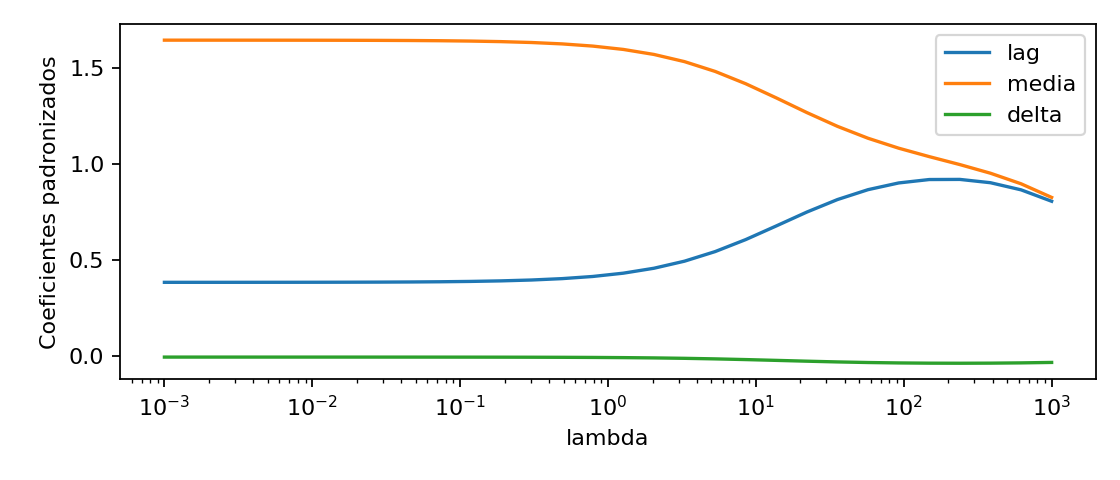
\includegraphics[width=.56\linewidth]{ridge.png}
\caption{Trajetórias dos coeficientes de Ridge em função da penalidade L2.}\label{fig:ridge}\end{figure}

O elevado $R^2$ reflete, em parte, a persistência da ordem de grandeza específica de cada série UF--evento. Não equivale a prever episódios excepcionais nem mede o efeito causal de políticas públicas. As métricas são calculadas após a transformação da resposta; a interpretação na escala original requer transformação inversa e análise de erro próprio.

\section{Etapa 3: Fundamentos de probabilidade}
Definem-se $A=\{\text{volume alto}\}$, $B=\{\text{aumento no mês anterior}\}$ e $C=\{\text{segundo semestre}\}$. Os quatro eventos atômicos do produto $A\times B$ são disjuntos e exaustivos: suas frequências relativas somam 1. As probabilidades são estimadas em observações de treinamento, com $P(A)=0.2244$, $P(B)=0.3296$ e $P(A\cap B)=0.0883$. As marginais resultam das somas de linhas e colunas, e $P(A\cup B)=P(A)+P(B)-P(A\cap B)=0.4657$.

\begin{table}[H]\centering\small\caption{Distribuição conjunta empírica de $A$ e $B$ (treinamento).}
\begin{tabular}{lrr}\toprule & $B=0$ & $B=1$ \\ \midrule
$A=0$ & 0.5343 & 0.2413 \\
$A=1$ & 0.1361 & 0.0883 \\
\bottomrule\end{tabular}\end{table}

A regra da cadeia $P(A,B,C)=P(A\mid B,C)P(B\mid C)P(C)$ reproduziu $P(A,B,C)=0.0323$ pelo produto dos termos condicionais. Pelo teorema de Bayes, $P(A\mid B)=P(B\mid A)P(A)/P(B)=0.2679$. A igualdade permite interpretar uma evidência observacional de forma diagnóstica, sem supor causalidade. A independência condicional dos atributos $B$ (aumento prévio) e $C$ (semestre) foi examinada \emph{dada a classe} $A$. Os desvios entre $P(B,C\mid A)$ e $P(B\mid A)P(C\mid A)$ foram de 0,0182 para $A=0$ e 0,0121 para $A=1$. Logo, a hipótese de independência condicional do Naive Bayes é uma aproximação, não uma identidade empírica.

A lógica de primeira ordem descreve relações e regras determinísticas, mas uma sentença clássica não atribui diretamente ``70\% de chance'' a um acontecimento. Para expressar tal grau de crença, emprega-se uma semântica probabilística adicional. Neste domínio, a incerteza diz respeito a contagens agregadas e qualidade de registro, não à propensão individual à prática de delito.

\section{Etapa 4: Aprendizado probabilístico e EM}
Para $x_i\in\{0,1\}$, a estimativa Bernoulli por máxima verossimilhança é $\hat\theta_{\mathrm{MV}}=\sum x_i/n=0.2244$. Com prior $\mathrm{Beta}(2,2)$, a \emph{moda posterior} é $(\sum x_i+1)/(n+2)=0.2247$; ela é diferente da média posterior $(\sum x_i+2)/(n+4)=0.2250$. O Naive Bayes categórico foi implementado com Laplace, categoria para valores inéditos e verificação no mesmo teste da Etapa 1. Sua acurácia foi 87.07\%.

A elevada frequência de observações com $lag1=0$ pode levar uma gaussiana irrestrita à degeneração da variância, pois sua densidade em uma massa pontual cresce à medida que a variância diminui. Adotou-se um modelo \emph{hurdle}: zeros são massa discreta observada, enquanto valores positivos recebem uma mistura de duas gaussianas ajustadas em $\log(1+lag1)$. O estado oculto $Z$ distingue regimes de volume anterior positivo; a categoria zero não é uma gaussiana. As responsabilidades do E-step incorporam pesos, médias e variâncias, e a variância mínima é 0,05.

\begin{figure}[H]\centering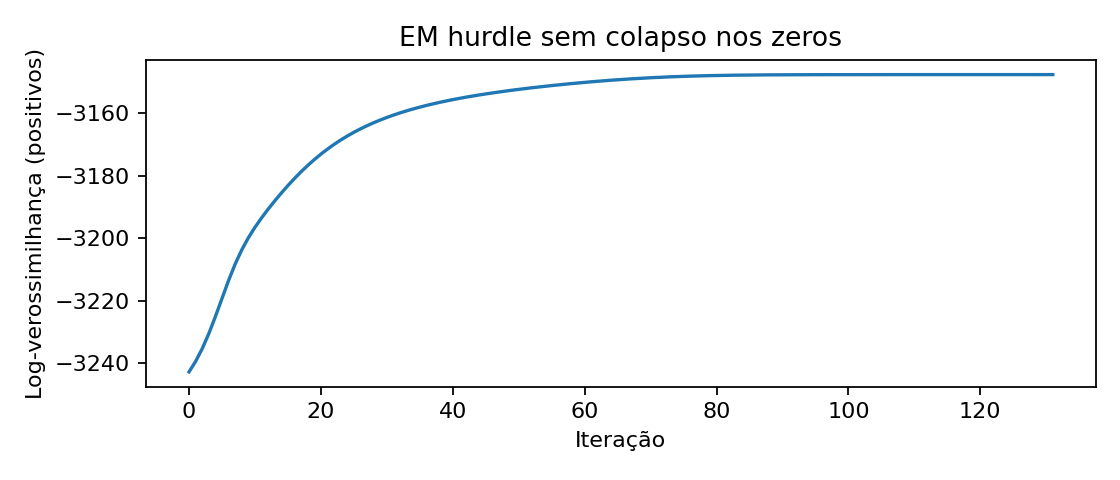
\includegraphics[width=.56\linewidth]{em_verossimilhanca.png}
\caption{Log-verossimilhança da mistura positiva ao longo do EM.}\label{fig:em}\end{figure}

Na amostra de treino, 19.69\% dos valores de $lag1$ eram zero. O EM terminou em 132 iterações, com variâncias 0.1411 e 2.1427, sem diminuição significativa de log-verossimilhança. O NB com $Z$ teve acurácia 87.64\%, diferença de 0.58 ponto percentual ante o NB puro (três acertos líquidos em 518 casos). Na comparação pareada ocorreram 11 correções e oito perdas, com $p=0.6476$ no teste exato de McNemar; portanto, não há evidência estatística suficiente de superioridade. Além disso, $Z$ deriva do histórico e pode ser redundante com os demais atributos. A trajetória de convergência e os parâmetros estão salvos em JSON e na Figura~\ref{fig:em}.

\section{Etapa 5: Rede Bayesiana e d-separação}
A rede contém seis nós: \texttt{uf} (27 estados), \texttt{semestre2} (2), \texttt{lag\_alto} (2), \texttt{regime\_em} (3), \texttt{alto} (2) e \texttt{crescimento} (2). O histórico e a classificação das etapas 1 e 4 são reutilizados diretamente. Cada CPT foi estimada com suavização de Laplace \emph{somente no treino}, e consultas condicionais são calculadas por enumeração própria. As arestas são hipóteses de fatoração associativa, não afirmações de causalidade.

\begin{figure}[H]\centering
\resizebox{.98\linewidth}{!}{%
\begin{tikzpicture}[>=Stealth,scale=.88,every node/.style={transform shape},
 n/.style={draw=black!60,fill=gray!8,rounded corners,align=center,minimum width=2.0cm,minimum height=.55cm,font=\small}]
\node[n] (uf) at (0,2.3) {UF}; \node[n] (sem) at (8,2.3) {Semestre};
\node[n] (lag) at (-1,.9) {Volume anterior}; \node[n] (reg) at (2,.9) {Regime EM};
\node[n] (alto) at (3.5,-.6) {Volume alto}; \node[n] (cre) at (7,-1.7) {Crescimento};
\draw[->] (uf)--(lag); \draw[->] (uf)--(reg); \draw[->] (uf) to[bend left=20] (alto);
\draw[->] (lag)--(alto); \draw[->] (reg)--(alto); \draw[->] (alto)--(cre); \draw[->] (sem)--(cre);
\end{tikzpicture}}
\caption{DAG proposto: o crescimento é um colisor entre semestre e volume alto.}\label{fig:dag}
\end{figure}

Para seis variáveis com as cardinalidades observadas, a conjunta irrestrita exige 1295 parâmetros livres, contra 274 no DAG: economia de 1021. Pela d-separação, \texttt{semestre2} e \texttt{alto} são independentes na rede sem observar o colisor; $P(S=1)=0.3698$ e $P(S=1\mid alto=1)=0.3698$. Ao condicionar em \texttt{crescimento}, a probabilidade torna-se 0.3036 se crescimento for 0 e 0.4217 se for 1. Essa alteração é uma demonstração numérica do efeito do colisor, não prova de causalidade real.

A enumeração própria calcula consultas exatas na rede discreta. A implementação disponibiliza a comparação de dez consultas com \texttt{pgmpy.VariableElimination} durante a execução da Etapa 5. A concordância numérica deve ser verificada no ambiente de reprodução com a biblioteca instalada; não se toma uma diferença registrada em outra execução como evidência de validação local.

\section{Etapa 6: Inferência fuzzy e integração}
As probabilidades $P(alto=1\mid e)$ e $P(crescimento=1\mid e)$ produzidas pela Etapa 5 alimentam o sistema Mamdani. Os antecedentes possuem conjuntos triangulares baixo, médio e alto (risco) e estável e crescente (tendência); a saída entre 0 e 100 tem classes baixa, média e alta. Empregam-se cinco regras: baixo e estável$\to$baixa; (baixo e crescente) ou (médio e estável)$\to$média; médio e crescente$\to$alta; alto e crescente$\to$alta; e alto e estável$\to$média. Assim, a tendência influencia até mesmo observações de risco alto: volume elevado porém estável mantém prioridade média de acompanhamento, enquanto crescimento associado a risco elevado produz prioridade alta.

A inferência própria usa mínimos no operador E, máximo no OU e na agregação, implicação por recorte e centroide para defuzzificação. O cruzamento efetivo foi aplicado às 518 linhas de teste, com a previsão ID3 preservada como comparador de interpretação, produzindo \textbf{169 pares distintos} de entradas probabilísticas e 12 divergências de classificação entre limiar rígido em $0,5$ e decisão fuzzy binarizada em 50. O mapa de sensibilidade de 11 por 11 (Figura~\ref{fig:fuzzy}) produziu 34 divergências em 121 combinações, inclusive próximas à fronteira. A previsão ID3 da Etapa 1 divergiu da decisão Bayesiana rígida em \textbf{39} linhas e da classificação fuzzy em \textbf{39} linhas; essas discordâncias permitem inspecionar casos limítrofes e integrar a decisão simbólica à análise final sem circularidade. A Etapa 6 disponibiliza comparação com \texttt{scikit-fuzzy} em 25 configurações; a diferença máxima deve ser calculada na execução com a biblioteca instalada. Dessa forma, a consistência da implementação pode ser auditada sem atribuir resultados a verificações não realizadas no mesmo ambiente.

\begin{figure}[H]\centering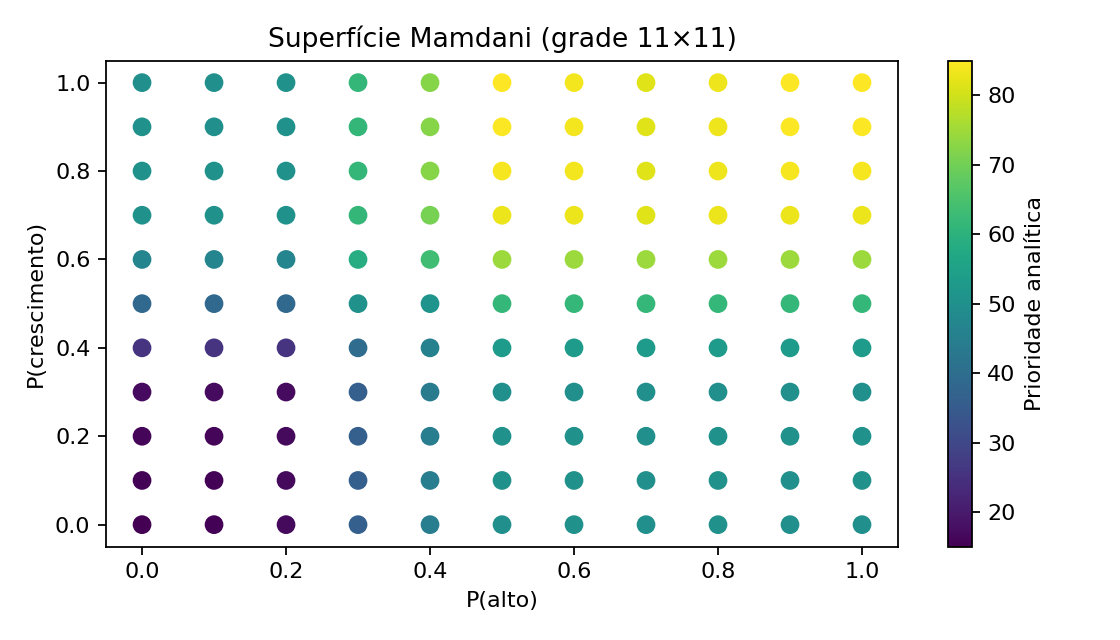
\includegraphics[width=.56\linewidth]{fuzzy_superficie.png}
\caption{Prioridade contínua nas 121 combinações de risco e tendência.}\label{fig:fuzzy}\end{figure}

A maior vantagem da abordagem fuzzy é descrever variações graduais em regiões limítrofes, não garantir acurácia superior. A previsão simbólica e as probabilidades do modelo são apresentadas conjuntamente ao especialista. A transparência das regras permite revisão especializada e explicação dos limiares; não se deve traduzir a saída em classificação de cidadãos, alocação policial automatizada ou inferências sobre causalidade sem avaliação adicional.

\section{Integração e considerações finais}
\begin{figure}[H]\centering
\resizebox{.98\linewidth}{!}{%
\begin{tikzpicture}[>=Stealth,node distance=2mm,
 b/.style={draw=black!55,rounded corners,align=center,minimum width=8.8cm,minimum height=.43cm,font=\footnotesize}]
\node[b] (x0) {Planilha VDE + estimativa IBGE 2026 $\to$ painel UF--evento--mês};
\node[b,below=of x0] (x1) {Etapa 1: ID3 $\to$ alto, UF, lag e baselines};
\node[b,below=of x1] (x2) {Etapa 2: regressões, Ridge e logística};
\node[b,below=of x2] (x3) {Etapa 3: conjunto, cadeia e Bayes};
\node[b,below=of x3] (x4) {Etapa 4: NB e EM $\to$ regime $Z$};
\node[b,below=of x4] (x5) {Etapa 5: DAG com UF, alto e $Z$ $\to$ probabilidades};
\node[b,below=of x5] (x6) {Etapa 6: Mamdani $\to$ prioridade estatística interpretável};
\foreach \a/\b in {x0/x1,x1/x2,x2/x3,x3/x4,x4/x5,x5/x6}{\draw[->] (\a)--(\b);}
\draw[->,dashed,red!65!black] (x1.east) to[bend left=42] node[right,font=\scriptsize,xshift=1mm]{alvo/UF} (x5.east);
\draw[->,dashed,red!65!black] (x1.east) to[bend left=58] (x6.east);
\draw[->,dashed,blue!70!black] (x4.west) to[bend right=32] node[left,font=\scriptsize,xshift=-1mm]{$Z$} (x5.west);
\end{tikzpicture}}
\caption{Fluxo completo: setas tracejadas correspondem a valores efetivamente reutilizados no código.}\label{fig:pipeline}\end{figure}

Em resposta à pergunta prática, o painel permite localizar combinações de UF, indicador e período com volumes classificados como elevados e examinar suas probabilidades e prioridades fuzzy. No treino, SP e RJ apresentaram proporções elevadas da classe \texttt{alto} (91,14\% e 90,41\%, respectivamente), mas isso reflete em parte o porte e o padrão de registros, e não demonstra que sejam os estados de maior risco populacional. A dimensão temporal é representada pelos meses observados e pela avaliação agosto--setembro; não há base para apontar um mês futuro como prioritário. Portanto, os resultados apoiam a seleção de situações para análise aprofundada, e não um ranking definitivo de risco por estado ou mês.

A integração emprega um painel estadual documentado, modelos simbólicos e probabilísticos, e um sistema de decisão graduada. A classificação principal é influenciada pelo porte e pelas práticas de registro das UFs, enquanto a série temporal contém apenas nove meses; por isso, as taxas mensais por população do IBGE foram examinadas em análise de sensibilidade, sem substituir o alvo principal. O controle do vazamento na definição do P75, a avaliação fora da amostra, a regularização do EM e as inferências condicionais são indispensáveis à interpretação responsável dos resultados. A prioridade fuzzy constitui apoio à análise estatística agregada, não fundamento automático para intervenção sobre pessoas.

\section{Interação com outras equipes do eixo P3}
Dentro do eixo de segurança pública, a equipe trocou perspectivas com o grupo que estuda a presença e a expansão de facções criminosas nos municípios do Amazonas. O registro abaixo reproduz o diálogo e a síntese produzida a partir dele.

\begin{list}{}{\setlength{\leftmargin}{.4cm}\setlength{\rightmargin}{0cm}\setlength{\topsep}{2pt}\setlength{\itemsep}{2pt}\setlength{\parsep}{0pt}}\footnotesize
\item[] \textbf{Equipe 5 --- Segurança Pública:} Nosso projeto utiliza indicadores oficiais de segurança pública para aplicar técnicas de Inteligência Artificial, incluindo árvores de decisão, regressão, inferência probabilística, estimação estatística, redes Bayesianas e lógica fuzzy. Buscamos identificar situações de elevado volume de ocorrências que possam demandar maior atenção da gestão pública.
\item[] \textbf{Equipe --- Facções Criminosas no Amazonas:} Nosso estudo investiga a presença e a expansão de facções criminosas nos municípios do Amazonas. Utilizamos rótulos provenientes das Cartografias, 3\textsuperscript{a} e 4\textsuperscript{a} edições, e atributos extraídos do Banco VDE do SINESP/MJSP, abrangendo o período de 2020 a 2024. Também integramos informações populacionais do IBGE e indicadores externos do IBAMA, INPE e IBGE.
\item[] \textbf{Equipe 5 --- Segurança Pública:} Uma diferença importante entre os projetos está na unidade de análise. Trabalhamos com indicadores agregados por unidade federativa e período, enquanto vocês utilizam informações municipais. A granularidade municipal pode permitir análises territoriais mais específicas, embora exija cuidados adicionais com a qualidade e a integração dos dados.
\item[] \textbf{Equipe --- Facções Criminosas no Amazonas:} Exatamente. Nossa metodologia utiliza códigos municipais para integrar diferentes fontes. Além dos registros de violência, consideramos variáveis territoriais e ambientais que podem contribuir para investigar associações com a presença de facções. Essas associações, entretanto, não devem ser interpretadas automaticamente como relações causais.
\item[] \textbf{Equipe 5 --- Segurança Pública:} Essa abordagem oferece uma perspectiva complementar à nossa. As técnicas probabilísticas e de classificação utilizadas em nosso trabalho poderiam, em estudos futuros, ser aplicadas a indicadores municipais para investigar padrões territoriais, desde que fossem realizados novos treinamentos e validações.
\item[] \textbf{Equipe --- Facções Criminosas no Amazonas:} Da mesma forma, a utilização de redes Bayesianas e lógica fuzzy poderia contribuir para representar incertezas e produzir classificações interpretáveis. Entretanto, seria necessário avaliar a qualidade dos rótulos e os riscos de generalização indevida dos resultados.
\item[] \textbf{Equipe 5 --- Segurança Pública:} Concluímos que os projetos são complementares: enquanto nossa pesquisa analisa indicadores agregados de segurança pública para apoiar o monitoramento, o estudo de vocês investiga padrões municipais relacionados à presença e à expansão de facções criminosas. A integração dessas perspectivas poderia fundamentar pesquisas futuras sobre análise territorial e apoio à decisão pública.
\end{list}

\textbf{Síntese.} A comparação evidencia a importância da granularidade territorial, da integração de bases oficiais, da interpretação probabilística e da validação dos modelos. Também demonstra que indicadores de violência e presença de organizações criminosas representam fenômenos distintos, que não devem ser tratados como equivalentes.

\begin{thebibliography}{9}\small
\bibitem{mj} BRASIL. Ministério da Justiça e Segurança Pública. \textit{Estatísticas de Segurança Pública: Base VDE 2026}. Disponível em: \url{https://www.gov.br/mj/pt-br/assuntos/sua-seguranca/seguranca-publica/estatistica}. Acesso em: 3 nov. 2026. Planilha fornecida para o trabalho.
\bibitem{ibge} IBGE. \textit{Estimativas da população residente no Brasil e Unidades da Federação com data de referência em 1$^{\circ}$ de julho de 2026}. Atualização em 29 out. 2026. Disponível em: \url{https://ftp.ibge.gov.br/Estimativas_de_Populacao/Estimativas_2026/POP2026_20261029.pdf}. Acesso em: 3 nov. 2026.
\bibitem{rn} RUSSELL, S.; NORVIG, P. \textit{Artificial Intelligence: A Modern Approach}. 4. ed. Pearson, 2020.
\bibitem{zadeh} ZADEH, L. A. Fuzzy sets. \textit{Information and Control}, v. 8, n. 3, p. 338--353, 1965.
\bibitem{huller} HÜLLERMEIER, E. Fuzzy machine learning and data mining. \textit{WIREs Data Mining and Knowledge Discovery}, v. 1, n. 4, p. 269--283, 2011.
\end{thebibliography}
\appendix
\section{Prompts utilizados em outra IA}
Prompts, na ordem em que foram enviados a outra ferramenta de IA durante o desenvolvimento:
\begin{enumerate}\small\setlength{\itemsep}{1pt}\setlength{\topsep}{1pt}\setlength{\parsep}{0pt}
\item ``Estou fazendo um trabalho de Fundamentos de IA sobre Segurança Pública, utilizando dados do MJSP e do IBGE. O professor pediu um projeto com seis etapas, desde árvore de decisão até lógica fuzzy. Me ajude a organizar a estrutura inicial do projeto em Python, separando os notebooks de cada etapa e os arquivos auxiliares. Também quero deixar tudo organizado para futuramente colocar no GitHub.''
\item ``Agora vamos começar a implementação. Quero utilizar os dados de segurança pública do MJSP e relacionar com os dados populacionais do IBGE. Primeiro, faça o tratamento e a organização desses dados, criando uma base que possamos utilizar nas próximas etapas. Depois implemente uma árvore de decisão do zero utilizando entropia e ganho de informação, e compare os resultados com a biblioteca scikit-learn.''
\item ``Vamos continuar o trabalho com as próximas etapas. Implemente regressão linear, regressão multivariada com gradiente descendente, regularização Ridge e regressão logística. Depois, desenvolva a parte de probabilidade, trabalhando com distribuição conjunta, probabilidades condicionais e Teorema de Bayes. Organize as explicações e os cálculos dentro dos notebooks.''
\item ``Agora quero desenvolver a parte de aprendizado probabilístico. Implemente MLE, MAP e um classificador Naive Bayes do zero. Também precisamos implementar o algoritmo EM com dois componentes, mostrando as etapas de expectativa e maximização e gerando um gráfico da evolução da log-verossimilhança. Compare os resultados dos modelos.''
\item ``Vamos desenvolver as duas últimas etapas do trabalho. Primeiro, crie uma rede Bayesiana com variáveis relacionadas à segurança pública, incluindo o DAG, as tabelas de probabilidades condicionais e a inferência por enumeração. Depois implemente um sistema de lógica fuzzy utilizando o modelo Mamdani, com funções de pertinência e regras Se-Então. Quero que as probabilidades da rede Bayesiana sejam utilizadas como entradas do sistema fuzzy.''
\item ``Agora que as seis etapas estão implementadas, quero integrar tudo em um pipeline completo. Organize os arquivos auxiliares, crie um script para executar todas as etapas na ordem correta e outro para verificar se está tudo funcionando. Também organize o README com as instruções de execução e deixe o projeto pronto para ser enviado ao GitHub. Verifique se os notebooks e os arquivos estão organizados e se as etapas estão conectadas corretamente.''
\end{enumerate}
\section{Reprodução e verificação}
A execução das seis etapas é automatizada por \texttt{python scripts/run\_all.py}, com semente 42. O módulo \texttt{scripts/verify\_project.py} verifica dados, invariantes matemáticos e PDF, e a opção \texttt{--run-notebooks} também reexecuta os notebooks com \texttt{nbclient}. As fontes possuem checksums SHA-256. As comparações com \texttt{pgmpy} e \texttt{scikit-fuzzy} são executadas nos notebooks 5 e 6.
\end{document}
